%%%%%%%%%%%%%%%%%%%%%%%%%%%%%%%%%%%%%%%%%%%%%%%%%%%%%%%%%%%%%%%%%%%%%%%%%%%
%% Trim Size: 9.75in x 6.5in
%% Text Area: 8in (include Runningheads) x 5in
%% ws-m3as.tex   :   28-9-2018
%% Tex file to use with ws-m3as.cls written in Latex2E.
%% The content, structure, format and layout of this style file is the
%% property of World Scientific Publishing Co. Pte. Ltd.
%% Copyright 2018 by World Scientific Publishing Co.
%% All rights are reserved.
%%%%%%%%%%%%%%%%%%%%%%%%%%%%%%%%%%%%%%%%%%%%%%%%%%%%%%%%%%%%%%%%%%%%%%%%%%%%
%

\documentclass{ws-m3as}

\begin{document}

\markboth{Authors' Names}{Instructions for Typing Manuscripts (Paper's Title)}

%%%%%%%%%%%%%%%%%%% Publisher's Area please ignore %%%%%%%%%%%%%%%%%%%%%%%
%
\catchline{}{}{}{}{}
%
%%%%%%%%%%%%%%%%%%%%%%%%%%%%%%%%%%%%%%%%%%%%%%%%%%%%%%%%%%%%%%%%%%%%%%%%%%

\title{Instructions for typesetting manuscripts\\
using \LaTeX2e\footnote{For the title, try not to
use more than 3 lines. Typeset the title in 10 pt
Times Roman  and boldface.} }

\author{First Author\footnote{Typeset names in 8 pt Roman. Use the footnote to indicate the
present or permanent address of the author.}}

\address{University Department, University Name, Address\\
City, State ZIP/Zone,
Country\footnote{State completely without abbreviations, the
affiliation and mailing address, including country. Typeset in 8 pt
Times italic.}\\
first\_author@university.edu}

\author{Second Author}

\address{Group, Laboratory, Address\\
City, State ZIP/Zone, Country\\
second\_author@group.com}

\maketitle

\begin{history}
\received{(Day Month Year)}
\revised{(Day Month Year)}
%\accepted{(Day Month Year)}
\comby{(xxxxxxxxxx)}
\end{history}

\begin{abstract}
Abstract is required and should summarize, in less
than 300 words, the context, content and conclusions of the
paper. It should not contain any references or displayed
equations.  Textwidth of the abstract should be 4.5 inches.
\end{abstract}

\keywords{Keyword1; keyword2; keyword3.}

\ccode{AMS Subject Classification: 22E46, 53C35, 57S20}

\section{General Appearance}	

Contributions to {\it Mathematical Models and Methods in Applied Sciences}
will be reformatted from the electronic file provided by the
authors. Blank (redundant) spaces should be minimized by careful
arrangement of tables and\break
figures.

\section{The Main Text}
Contributions are to be in English. Authors are encouraged to
have their contribution checked for grammar. Abbreviations
are allowed but should be spelt out in full when first used.
Integers ten and below are to be spelt out but type as (2+1)
dimensions.  Italicize foreign language phrases (e.g.~Latin, French).

The text should be in 10 pt Times Roman, single spaced with
baselineskip of 13~pt. Text area (excluding copyright block and folio)
is 6.9 inches high and 5 inches wide for the first page.
Text area (excluding running title) is 7.7 inches high and\break
5 inches wide for subsequent pages.  Final pagination and
insertion of running titles will be done by the publisher.

\section{Major Headings}
Major headings should be typeset in boldface with the first
letter of important words capitalized.

\subsection{Sub-headings}
Sub-headings should be typeset in boldface italic and capitalize
the first letter of the first word only. Section number to be in
boldface roman.

\subsubsection{Sub-subheadings}
Typeset sub-subheadings in medium face italic and capitalize the
first letter of the first word only. Section number to be in
roman.

\subsection{Numbering}
Sections, sub-sections and sub-subsections are to be numbered in
Arabic.  Sections and sub-sections in boldface while
sub-subsections in Roman.

\subsection{Lists of items}

Lists may be laid out with each item marked by a dot:
\begin{itemlist}
 \item item one,
 \item item two.
\end{itemlist}

Items may also be numbered in lowercase roman numerals:
\begin{romanlist}[(ii)]
\item item one
\item item two
\begin{romanlist}[(b)]
\item Lists within lists can be numbered with lowercase roman letters,
\item second item.
\end{romanlist}
\end{romanlist}

\section{Equations}
Displayed equations should be numbered consecutively in each
section, with the number set flush right and enclosed in
parentheses.
\begin{equation}
\mu(n, t) = {\sum^\infty_{i=1} 1(d_i < t,
N(d_i) = n)}{\int^t_{\sigma=0} 1(N(\sigma) = n)d\sigma}\, .\label{this}
\end{equation}
Equations should be referred to in abbreviated form,
e.g.~``Eq.~(\ref{this})'' or ``(4.1)''. In multiple-line
equations, the number should be given on the last line.

Displayed equations are to be centered on the page width.  Standard
English\break
letters like x are to appear as $x$ (italicized) in the text
if they are used as mathematical symbols. Punctuation marks are used
at the end of equations as if they appeared directly in the text.

Each section should start with a fresh set of equation numbers, for
example, if Sec.~4 ends with Eq.~(4.3), the first equation number in
Sec.~5 should be (5.1) instead of (5.4).

\begin{theorem}\label{thm1}
Theorems$,$ lemmas$,$ etc. are to be numbered
consecutively in the paper or in each section. Use italic for the
body and upper and lower case boldface$,$ for the declaration.
\end{theorem}

\begin{lemma}[Optional Title]\label{lem1}
Theorems$,$ lemmas$,$ etc. are to be numbered
consecutively in the paper or in each section. Use italic for the
body and upper and lower case boldface$,$ for the declaration.
\end{lemma}

\begin{proof}
The word `Proof' should be in boldface. Proofs
should end with a box.
\end{proof}

\section{Illustrations and Photographs}
Figures are to be inserted in the text nearest their first
reference. eps files or postscript files are preferred. If
photographs are to be used, only black and white ones are acceptable.

\begin{figure}[pb]
\centerline{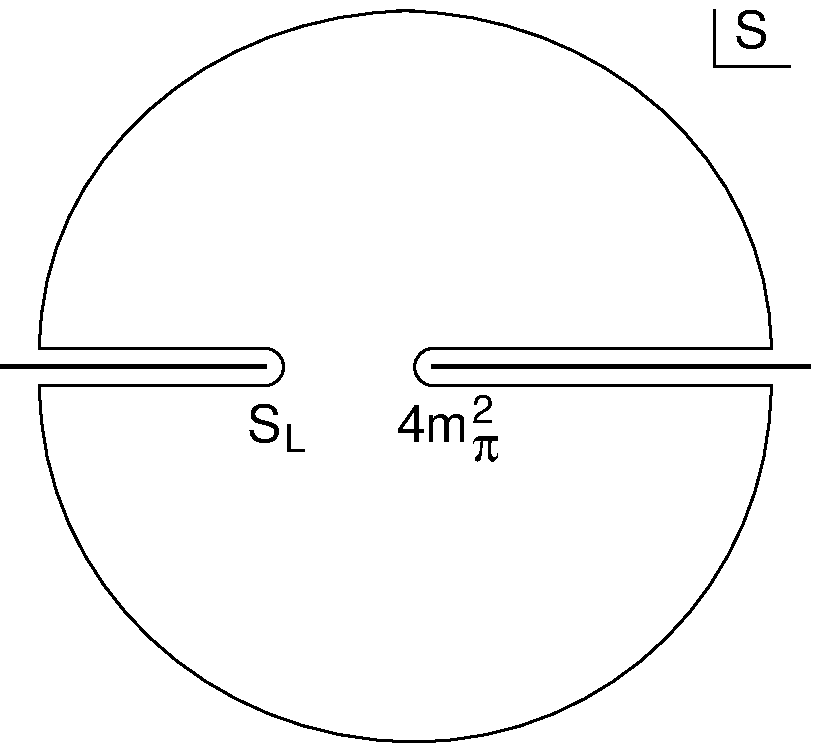
\includegraphics[width=1.8in]{m3asf1}}
\vspace*{8pt}
\caption{A schematic illustration of dissociative recombination. The
direct mechanism, 4m$^2_\pi$ is initiated when the
molecular ion S$_{\rm L}$ captures an electron with kinetic energy.}
\end{figure}

Figures are to be sequentially numbered in Arabic numerals.
Centralize the caption and place it below the figure.
Typeset in 8 pt Times Roman with
baselineskip of 10~pt. Use double spacing between a
caption and the text that follows immediately.

Previously published material must be accompanied by written
permission from the author and publisher.

\section{Tables}
Tables should be inserted in the text as close to the point of
reference as possible. Some space should be left above and below
the table.

\begin{table}[ht]
\tbl{Comparison of acoustic for frequencies for piston-cylinder problem.}
{\begin{tabular}{@{}cccc@{}} \toprule
Piston mass & Analytical frequency & TRIA6-$S_1$ model &
\% Error \\
& (Rad/s)$^{\rm a}$ & (Rad/s)$^{\rm b}$ \\ \colrule
1.0\hphantom{00} & \hphantom{0}281.0 & \hphantom{0}280.81 & 0.07 \\
0.1\hphantom{00} & \hphantom{0}876.0 & \hphantom{0}875.74 & 0.03 \\
0.01\hphantom{0} & 2441.0 & 2441.0\hphantom{0} & 0.0\hphantom{0} \\
0.001 & 4130.0 & 4129.3\hphantom{0} & 0.16\\ \botrule
\end{tabular}}
\begin{tabnote}
Table notes
\end{tabnote}
\begin{tabfootnote}
\tabmark{a} Table footnote A\\
\tabmark{b} Table footnote B
\end{tabfootnote}
\end{table}

Tables should be numbered sequentially in the text in Arabic
numerals. Captions are to be centralized above the tables.
Typeset tables and captions in 8 pt Times Roman with
baselineskip of 10 pt.

If tables need to extend over to a second page, the continuation
of the table should be preceded by a caption, e.g.~``Table 2.
({\it Continued})''

\section{Footnotes}
Footnotes should be numbered sequentially in superscript
alphabets.\footnote{Footnotes should be typeset in 8 pt
Times Roman at the bottom of the page.}

\section*{Note Added}
Should be placed before Acknowledgment.

\appendix

\section{Appendices}

Appendices should be used only when absolutely necessary. They
should come before the Acknowledgment. If there is more than one
appendix, number them alphabetically. Number displayed equations
in the way, e.g.~(\ref{that}), (A.2), etc.

\noindent
\begin{equation}
f(j\delta, i\delta) \cong \frac{\pi}{M} \sum^M_{n=1}
Q_{\theta_n} (j \cos \theta_n + i \sin \theta_n)\,. \label{that}
\end{equation}

\section*{Acknowledgment}
This section should come after the Appendices if any and should
be unnumbered. Funding information may also be included here.

\section*{References}
They are to be cited in the text in superscript
after comma and period (e.g.~word,\cite{am})
but before other punctuation marks like colons,
(e.g.~word\cite{lar}:) semi-colons and\break
question marks. If it is mentioned in the text as part of a sentence,
it should be of normal size, e.g.~see Ref.~\refcite{lar}.

\begin{thebibliography}{00}
%1
\bibitem{aiz} M. Aizenman and T. Bak, Convergence to equilibrium
in a system of reacting polymers, {\it Comm. Math. Phys.} {\bf 65}
(1979) 203--230.

%2
\bibitem{am} H. Amann, Coagulation--fragmentation
processes, {\it Arch. Rational Mech. Anal.} {\bf 151} (2000)
339--366.

%3
\bibitem{lar} L. Arlotti, A perturbation theorem for
positive contraction semigroups on $L^1$-spaces with applications to
transport equations and Kolmogorov's differential equations,
{\it Acta Appl. Math.} {\bf 23} (1991) 129--144.

%4
\bibitem{ba} L. Arlotti and J. Banasiak, Strictly substochastic
semigroups with application to conservative and
shattering solutions to fragmentation equations with mass loss,\break
{\it J. Math. Anal. Appl.} (2004), to appear.

%5
\bibitem{ge} L. Arlotti, N. Bellomo and E. De Angelis,
Generalized kinetic Boltzmann models: Mathematical structures and
applications, {\it Math. Mod. Meth. Appl. Sci.} {\bf 12} (2002)
571--596.

%6
\bibitem{ball} J. M. Ball and J. Carr, The discrete
coagulation--fragmentation equations: Existence, uniqueness and
density conservation, {\it J. Statist. Phys.} {\bf 61} (1990)
203--234.

%7
\bibitem{siak} J. Banasiak, On a diffusion-kinetic equation
arising in extended kinetic theory, {\it Math. Meth.
Appl. Sci.} {\bf 23} (2000) 1237--1256.

%8
\bibitem{jba} J. Banasiak, On an extension of Kato--Voigt
perturbation theorem for substochastic semigroups and its
applications, {\it Taiwanese J. Math.} {\bf 5}
(2001) 169--191.

%9
\bibitem{anas} J. Banasiak, On a non-uniqueness in
fragmentation models, {\it Math. Meth. Appl. Sci.}
{\bf 25} (2002) 541--556.

%10
\bibitem{boltz} J. Banasiak, On well-posedness of Boltzmann-like
semiconductor model, {\it Math. Mod. Meth. Appl. Sci.} {\bf 13}
(2003) 875--892.

%11
\bibitem{sol} J. Banasiak, Multiple solutions to linear kinetic
equations, {\it Trans. Th. Statist. Phys.} {\bf 32} (2003) 381--398.

%12
\bibitem{mcai} M. Cai, B. F. Edwards and H. Han,
Exact and asymptotic scaling solutions
for fragmentation with mass loss, {\it Phys. Rev.} {\bf A43} (1991) 656--662.

%13
\bibitem{nd} N. Dunford and J. T. Schwartz, {\it Linear Operators$,$
Part I\/$:$ General Theory} (John Wiley \& Sons, 1988).

%14
\bibitem{kje} K.-J. Engel and R. Nagel, {\it One-Parameter Semigroups
for Linear Evolution Equations}, Graduate Texts in Mathematics
(Springer-Verlag, 1999).

\end{thebibliography}

\end{document}

%%Typeout the superscript citation as:-
%%(1) word,\cite{aiz,am,lar} and word.\cite{aiz,am,lar}
%%(2) word\cite{ba}: word\cite{ba}; word\cite{ba}?
%%(3) See Ref.~\refcite{lar} --- to be cited at the text.